\documentclass[a4paper,10pt,fleqn]{article}
\usepackage{mathtext}
\usepackage[T2A]{fontenc}
\usepackage[utf8x]{inputenc}
\usepackage[english,ukrainian]{babel}
\usepackage{amsfonts,amsmath,stmaryrd}
\usepackage{indentfirst}
\usepackage[pdftex]{color,graphicx}
\usepackage{float}
\usepackage{subfig}
\usepackage[protrusion=true,expansion=true]{microtype}
%\usepackage{iwona}
%\usepackage{cmbright}
%\usepackage[math]{anttor}
\usepackage[condensed,math]{anttor}
%\usepackage[math]{kurier}
%\usepackage{literat}
    

\graphicspath{{./images/}}
\DeclareGraphicsRule{.jpeg}{.bmp}{}{}
\textwidth 16 cm
\textheight 24.5cm
\topmargin -1 cm
\evensidemargin 0 cm
\oddsidemargin 0 cm
\normalfont
\title{Результати тестування}
\author{Накрийко Андрій}

\begin{document}
\selectlanguage{ukrainian}
\maketitle

\newpage

\textbf{\textit{$\varepsilon$-функція}} вибору випадкової дії: 
\begin{itemize}
\item \textbf{linear} --- лінійно-спадна від $0.3$ до $0.0$ за 300000 ітерацій;
\item \textbf{spikes} --- пилкоподібно-спадна (погана) з 3-ма зубцями спад від $0.3$ до $0.01$ за 300000 ітерацій;
\end{itemize}

\textbf{\textit{$\eta$-функція}} кроку навчання для нейромережі:
\begin{itemize}
\item \textbf{linear} --- лінійно-спадна від $0.3$ до $0.01$ за 600000 ітерацій;
\item \textbf{exp} ---    експоненційно-спадна (погана) від $0.4$ до $0.01$ за 600000 ітерацій;
\item \textbf{spikes} --- пилкоподібно-спадна (погана) з 3-ма зубцями від $0.4$ до $0.01$ за 600000 ітерацій;
\end{itemize}

Далі параметри в формі: <\textit{структура нейромережі}> <\textit{$\eta$-функція}> <\textit{$\varepsilon$-функція}>.

\vspace*{1.5cm}

\begin{figure}[h]
  \centering
  \subfloat[spikes-функція (погана)]{\includegraphics[width=0.45\textwidth]{expSpikes_s3_bad}}\,
  \subfloat[exp-функція (погана)]{\includegraphics[width=0.45\textwidth]{exp_bad}} \\
  \caption{Погані функції}
\end{figure}

\begin{figure}[h]
  \centering
  \subfloat[spikes-функція (правильна)]{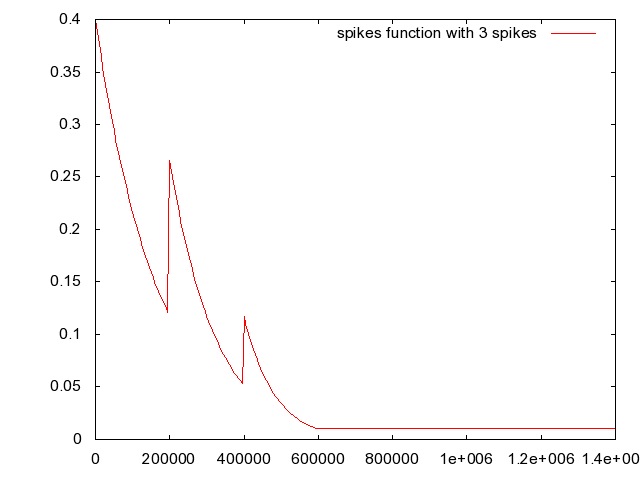
\includegraphics[width=0.45\textwidth]{expSpikes_s3}}\,
  \subfloat[exp-функція (правильна)]{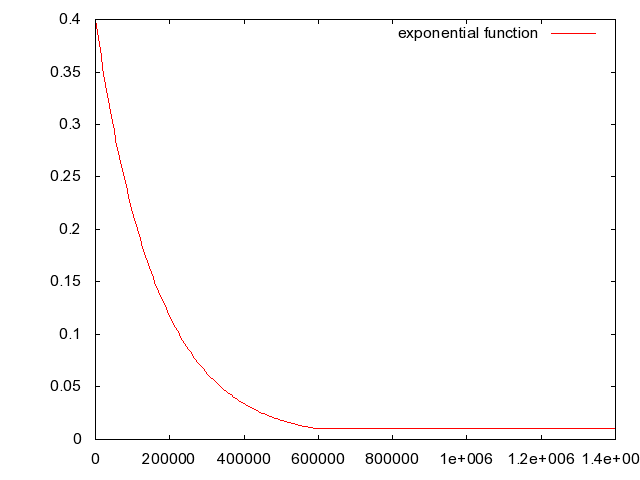
\includegraphics[width=0.45\textwidth]{exp}} \\
  \caption{Правильні функції (такі, якими б мали бути наведені вище)}
\end{figure}


\newpage

\begin{figure}
  \centering
  \subfloat{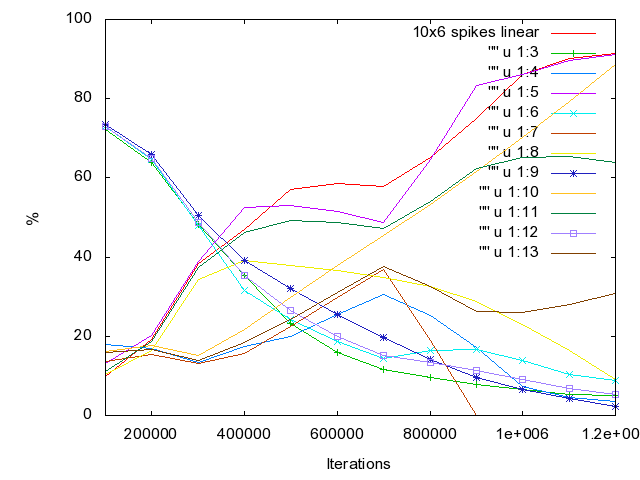
\includegraphics[width=0.4\textwidth]{10-6-spikes-linear}}\,
  \subfloat{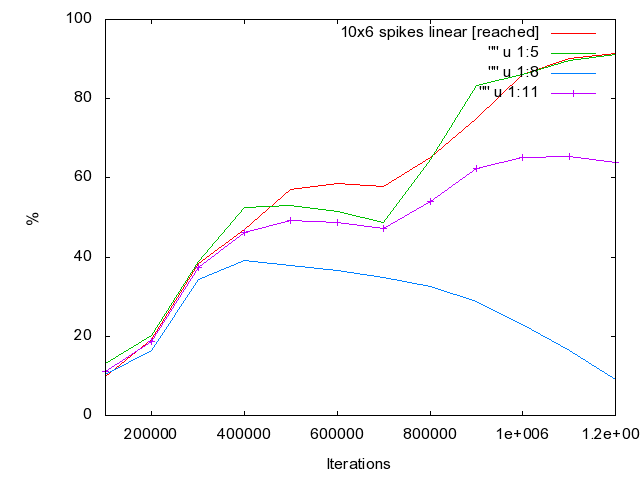
\includegraphics[width=0.4\textwidth]{10-6-spikes-linear_r}} \\
  \subfloat{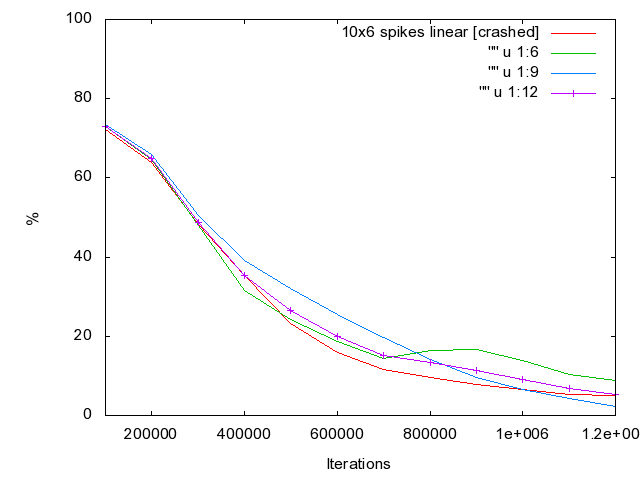
\includegraphics[width=0.4\textwidth]{10-6-spikes-linear_c}}\,
  \subfloat{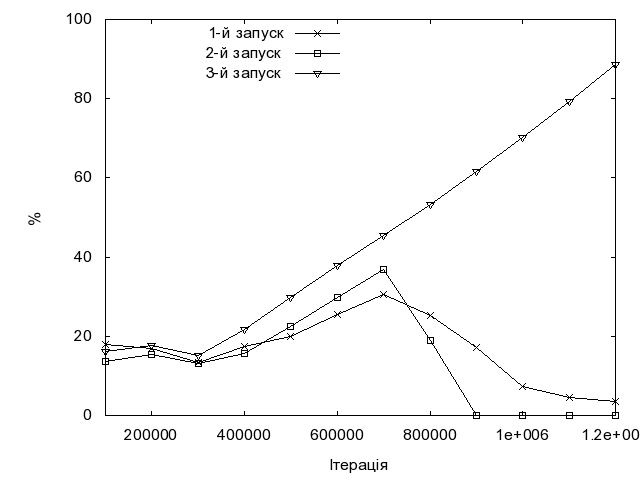
\includegraphics[width=0.4\textwidth]{10-6-spikes-linear_t}}
  \caption{10x6 spikes linear}
\end{figure}

\begin{figure}
  \centering
  \subfloat{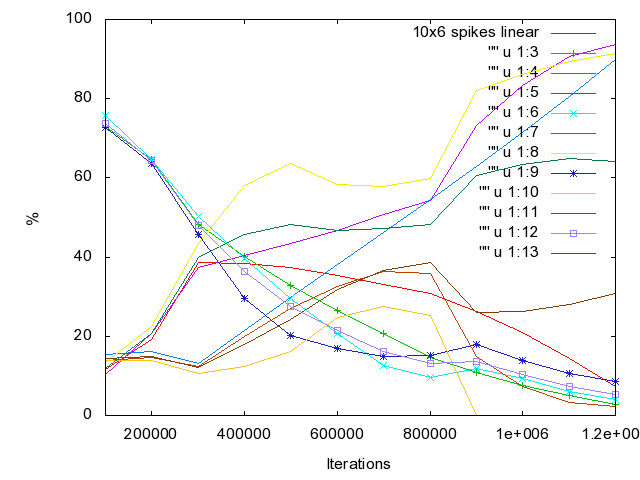
\includegraphics[width=0.4\textwidth]{10-6-spikes-linear2}}\,
  \subfloat{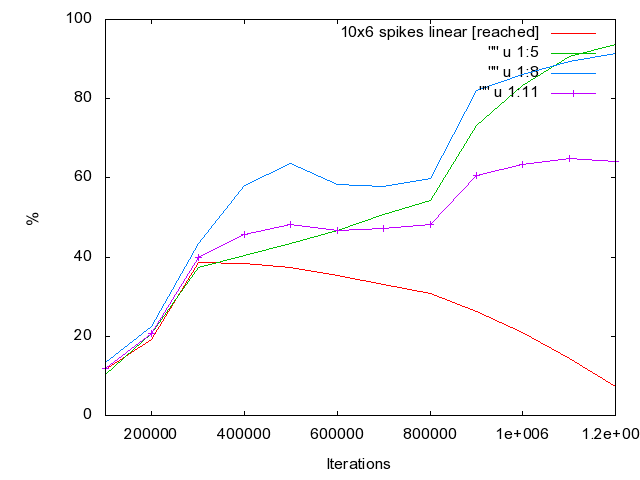
\includegraphics[width=0.4\textwidth]{10-6-spikes-linear2_r}} \\
  \subfloat{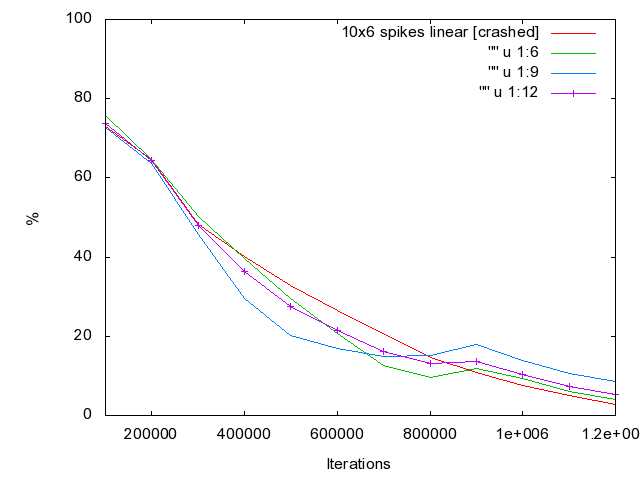
\includegraphics[width=0.4\textwidth]{10-6-spikes-linear2_c}}\,
  \subfloat{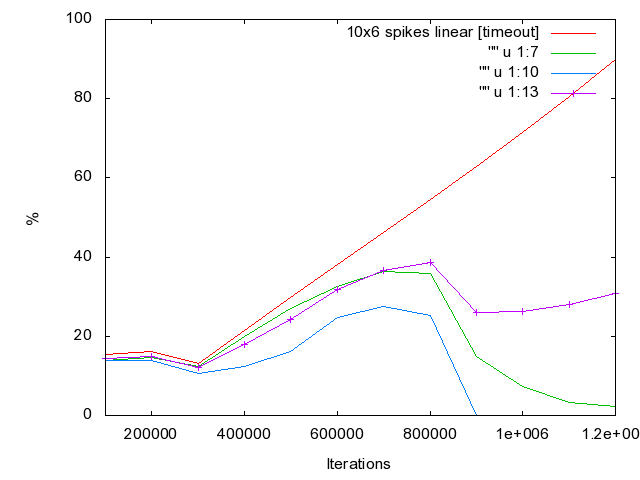
\includegraphics[width=0.4\textwidth]{10-6-spikes-linear2_t}}
  \caption{10x6 spikes linear}
\end{figure}

\begin{figure}
  \centering
  \subfloat{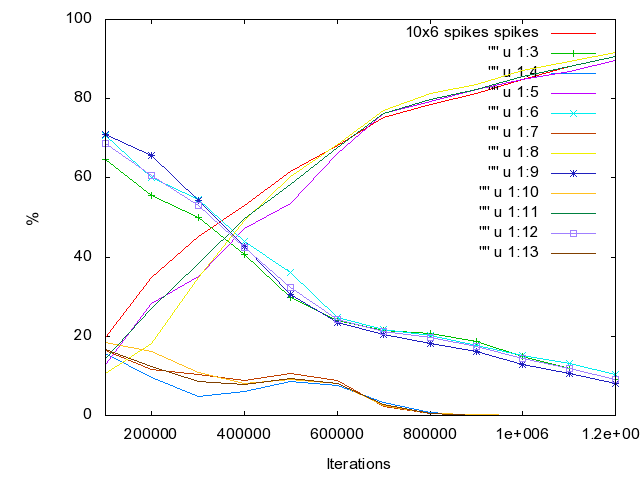
\includegraphics[width=0.4\textwidth]{10-6-spikes-spikes}}\,
  \subfloat{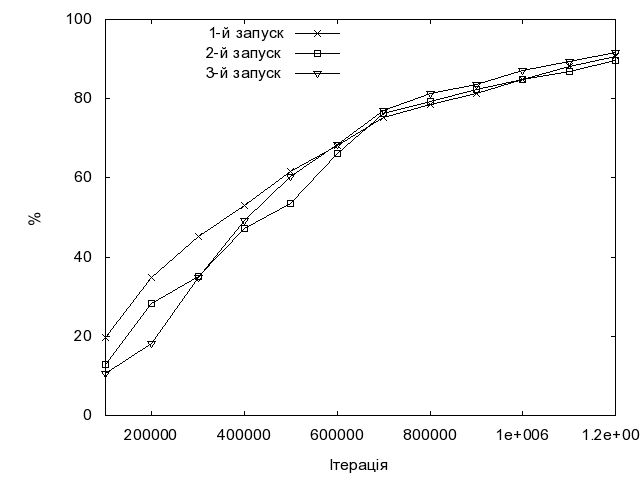
\includegraphics[width=0.4\textwidth]{10-6-spikes-spikes_r}} \\
  \subfloat{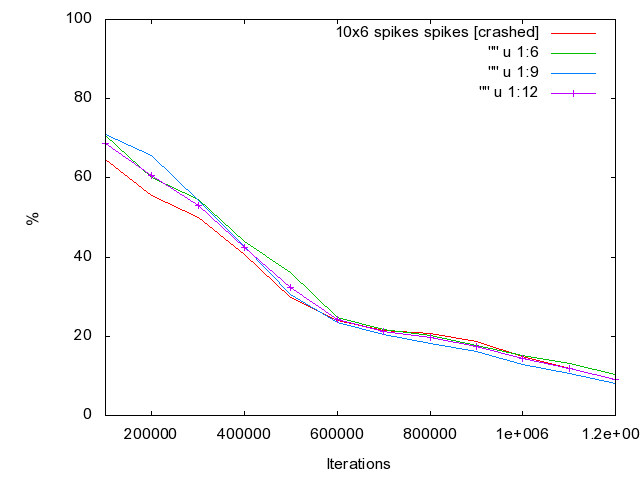
\includegraphics[width=0.4\textwidth]{10-6-spikes-spikes_c}}\,
  \subfloat{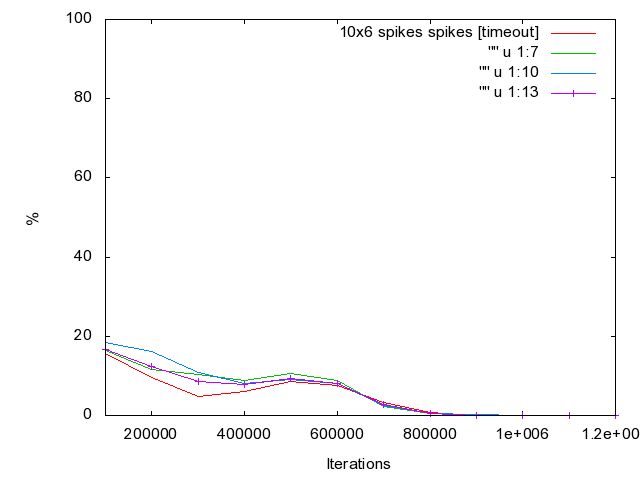
\includegraphics[width=0.4\textwidth]{10-6-spikes-spikes_t}}
  \caption{10x6 spikes spikes}
\end{figure}

\begin{figure}
  \centering
  \subfloat{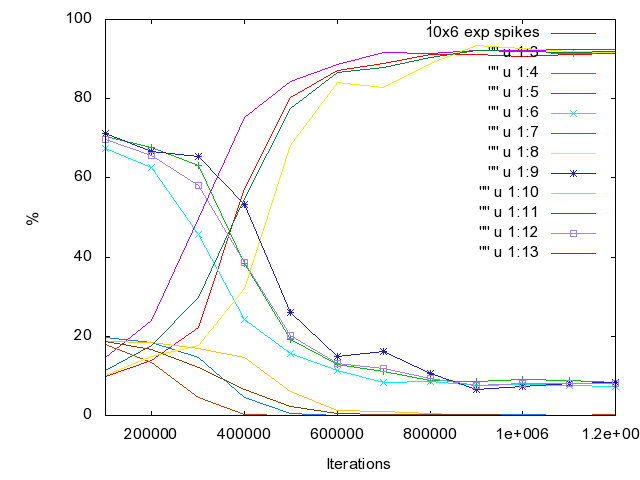
\includegraphics[width=0.4\textwidth]{10-6-exp-spikes}}\,
  \subfloat{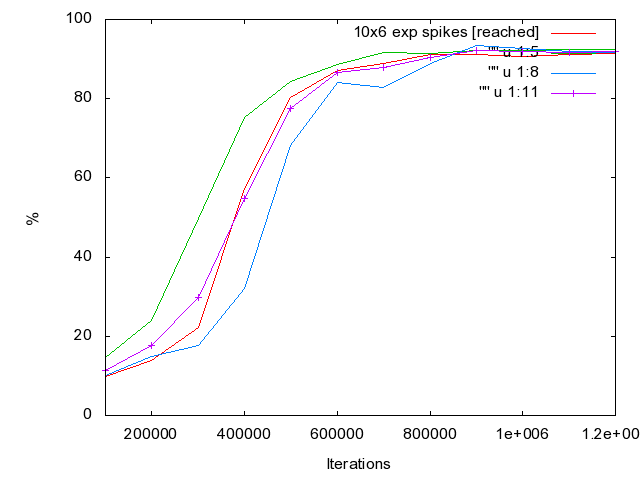
\includegraphics[width=0.4\textwidth]{10-6-exp-spikes_r}} \\
  \subfloat{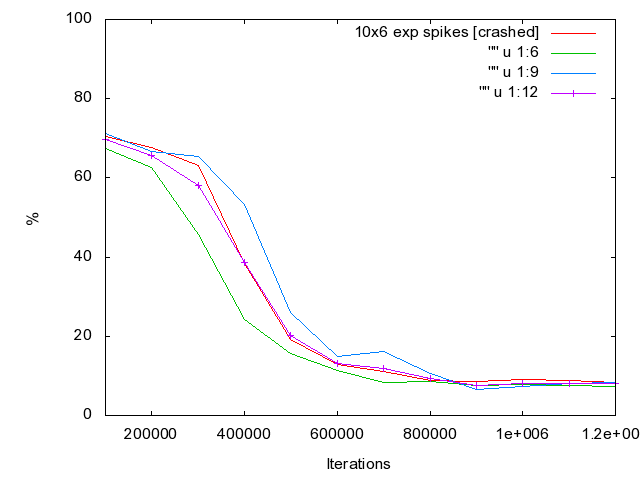
\includegraphics[width=0.4\textwidth]{10-6-exp-spikes_c}}\,
  \subfloat{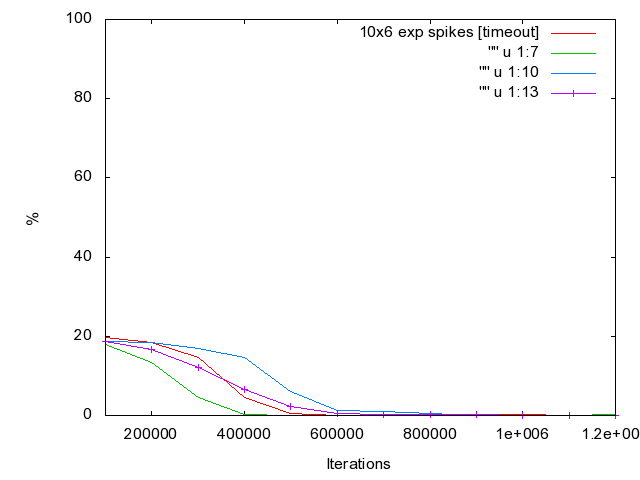
\includegraphics[width=0.4\textwidth]{10-6-exp-spikes_t}}
  \caption{10x6 exp spikes}
\end{figure}

\begin{figure}
  \centering
  \subfloat{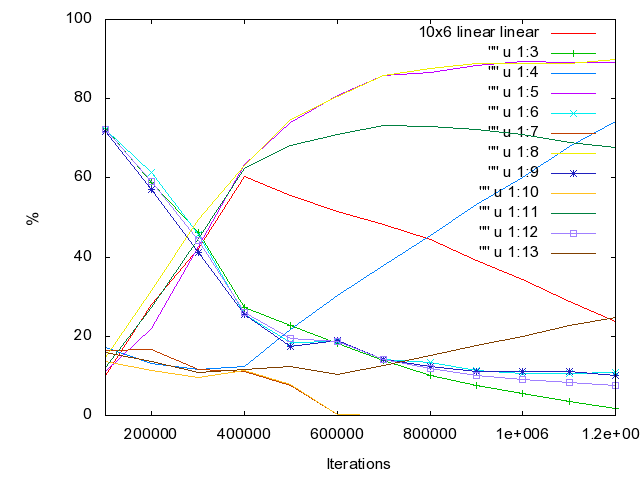
\includegraphics[width=0.4\textwidth]{10-6-linear-linear}}\,
  \subfloat{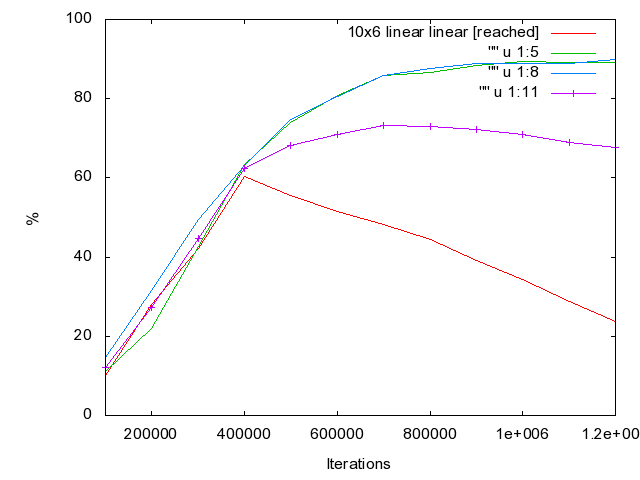
\includegraphics[width=0.4\textwidth]{10-6-linear-linear_r}} \\
  \subfloat{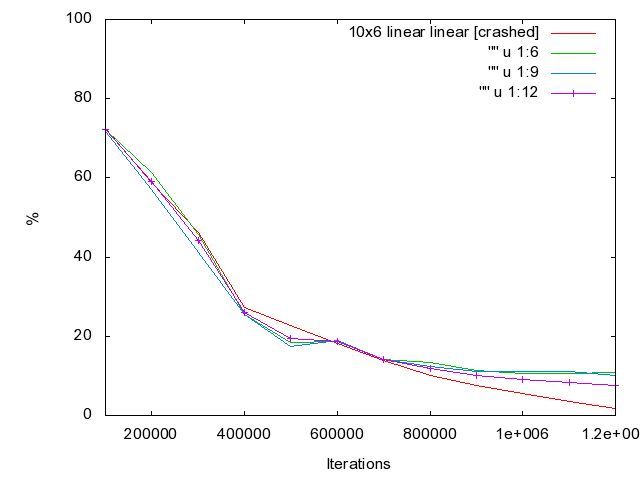
\includegraphics[width=0.4\textwidth]{10-6-linear-linear_c}}\,
  \subfloat{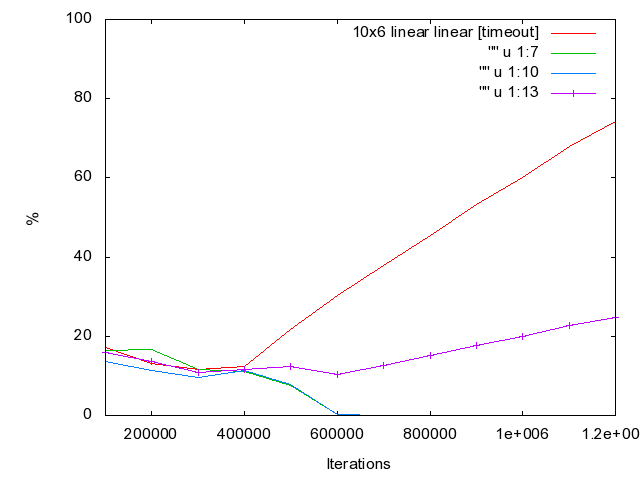
\includegraphics[width=0.4\textwidth]{10-6-linear-linear_t}}
  \caption{10x6 linear linear}
\end{figure}

\begin{figure}
  \centering
  \subfloat{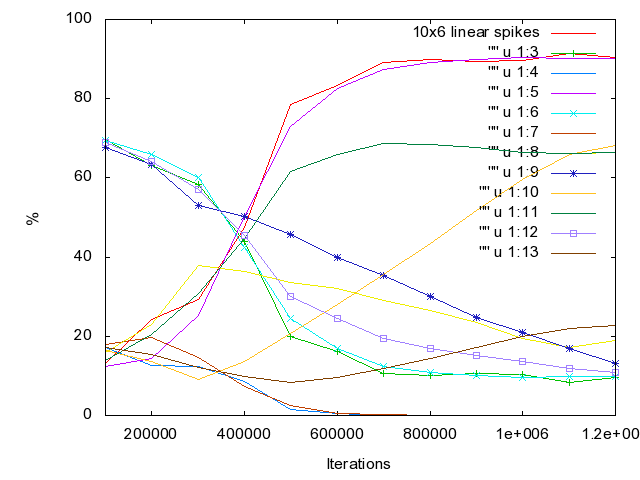
\includegraphics[width=0.4\textwidth]{10-6-linear-spikes}}\,
  \subfloat{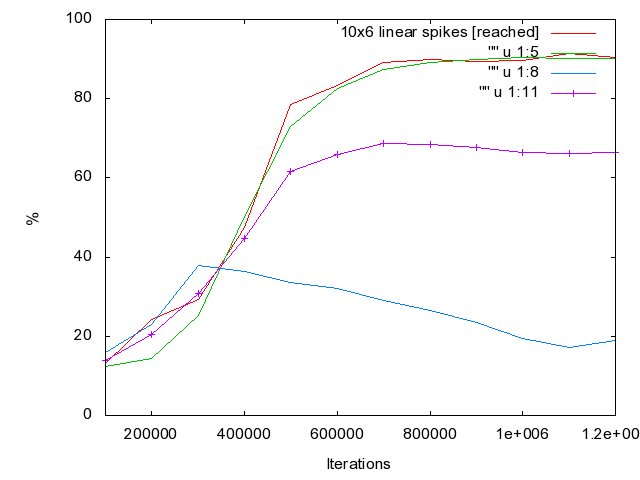
\includegraphics[width=0.4\textwidth]{10-6-linear-spikes_r}} \\
  \subfloat{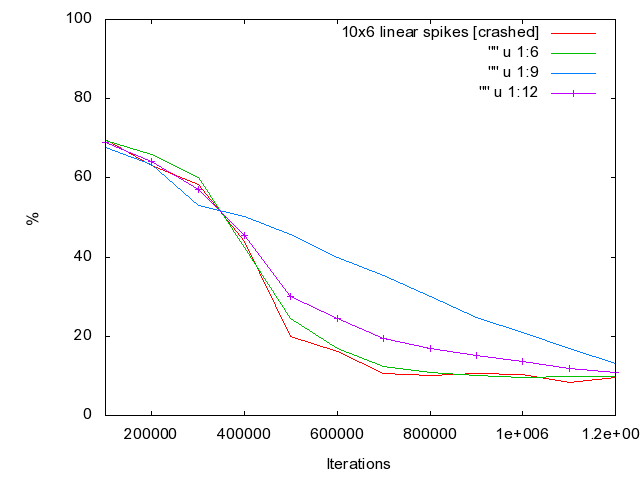
\includegraphics[width=0.4\textwidth]{10-6-linear-spikes_c}}\,
  \subfloat{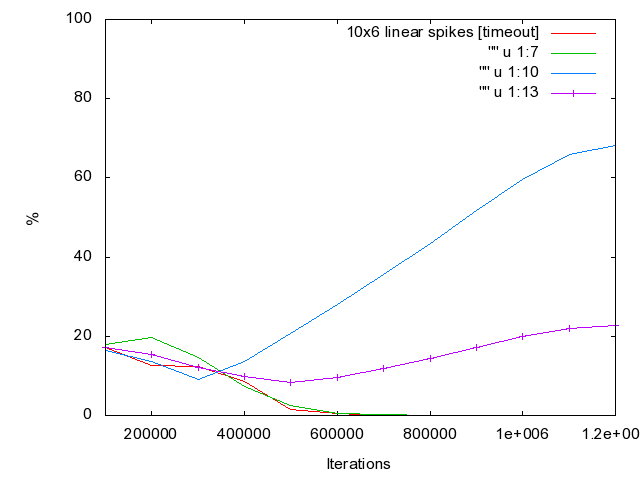
\includegraphics[width=0.4\textwidth]{10-6-linear-spikes_t}}
  \caption{10x6 linear spikes}
\end{figure}

\begin{figure}
  \centering
  \subfloat{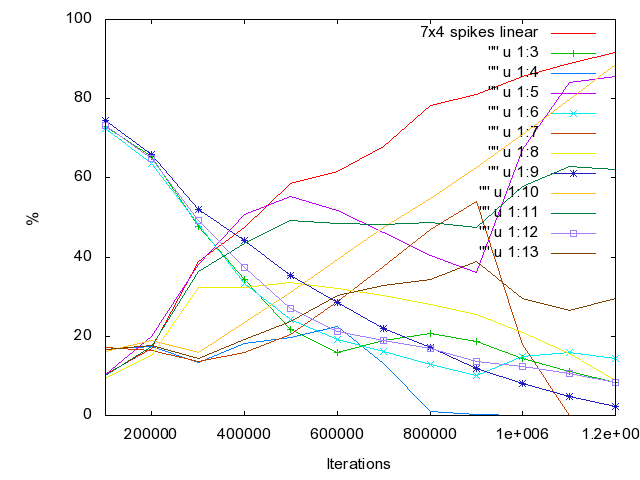
\includegraphics[width=0.4\textwidth]{7-4-spikes-linear}}\,
  \subfloat{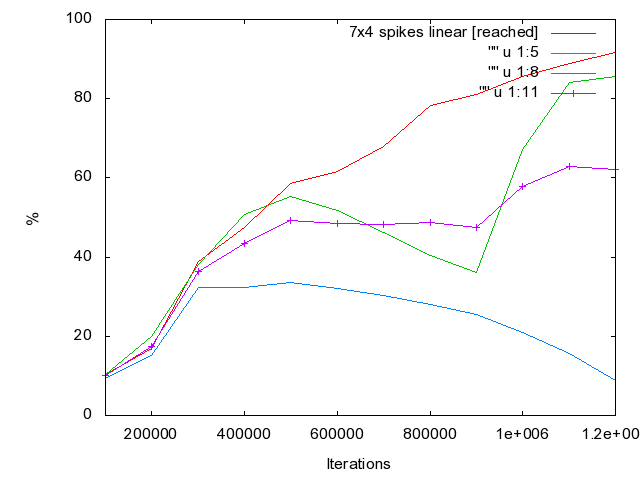
\includegraphics[width=0.4\textwidth]{7-4-spikes-linear_r}} \\
  \subfloat{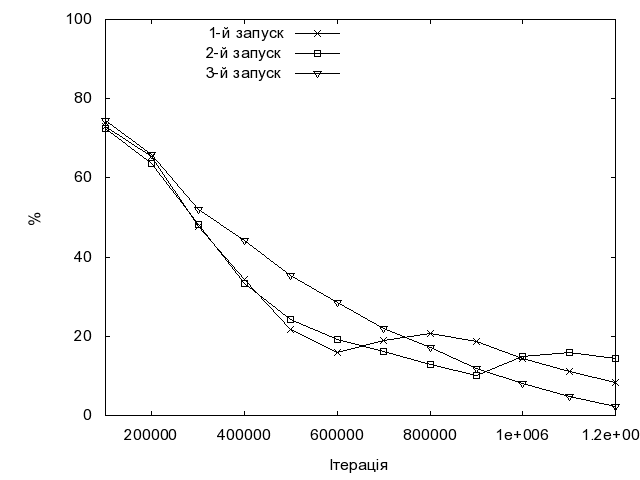
\includegraphics[width=0.4\textwidth]{7-4-spikes-linear_c}}\,
  \subfloat{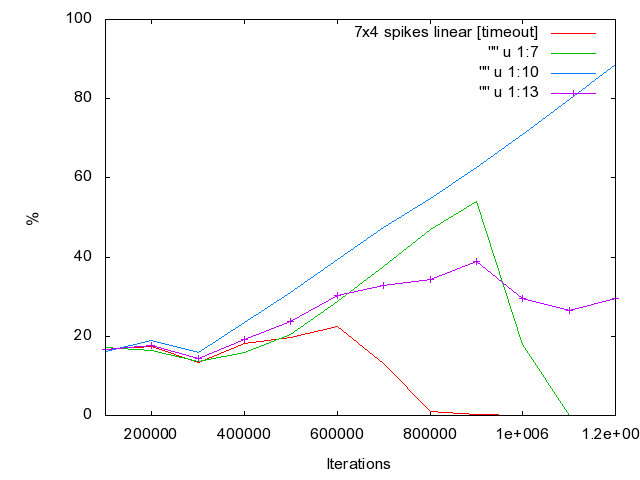
\includegraphics[width=0.4\textwidth]{7-4-spikes-linear_t}}
  \caption{7x4 spikes linear}
\end{figure}

\begin{figure}
  \centering
  \subfloat{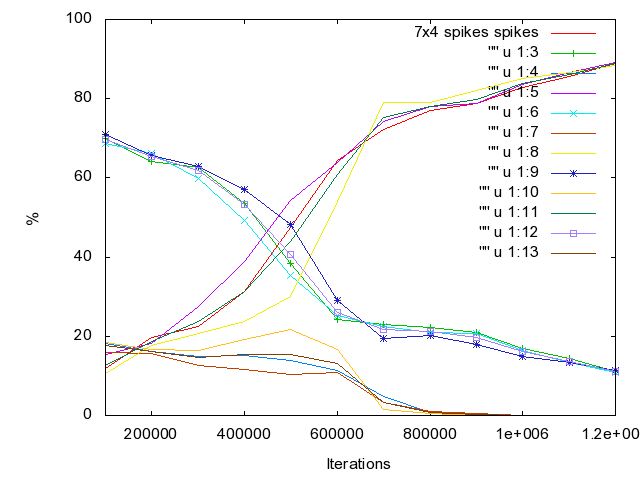
\includegraphics[width=0.4\textwidth]{7-4-spikes-spikes}}\,
  \subfloat{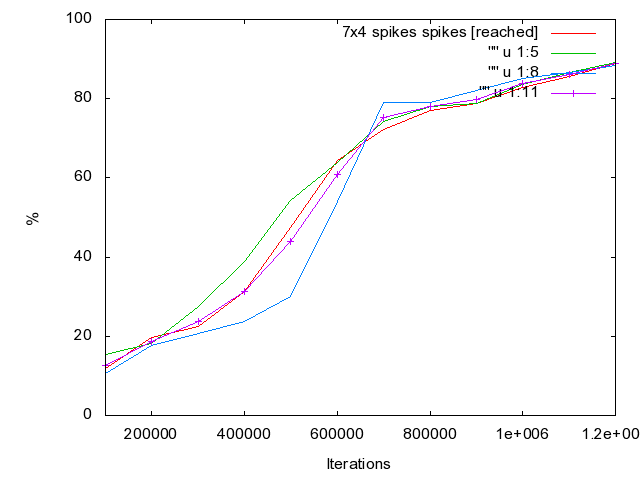
\includegraphics[width=0.4\textwidth]{7-4-spikes-spikes_r}} \\
  \subfloat{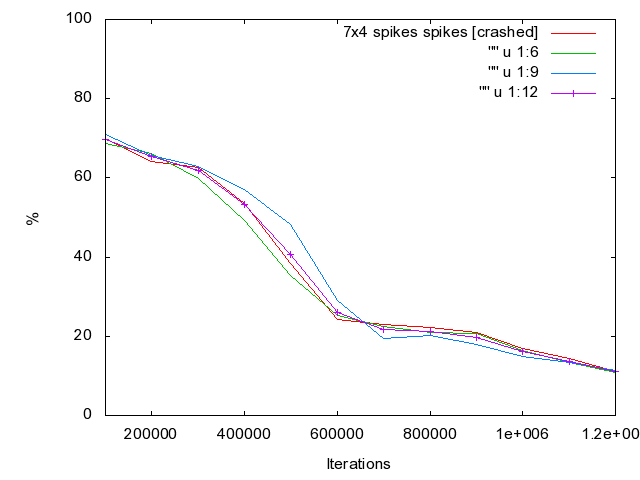
\includegraphics[width=0.4\textwidth]{7-4-spikes-spikes_c}}\,
  \subfloat{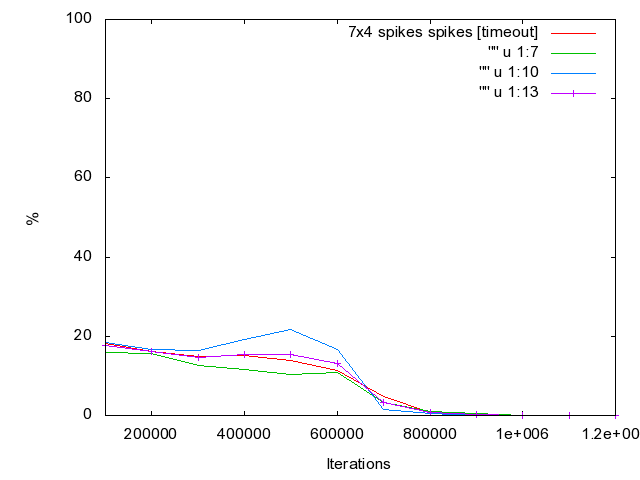
\includegraphics[width=0.4\textwidth]{7-4-spikes-spikes_t}}
  \caption{7x4 spikes spikes}
\end{figure}

\begin{figure}
  \centering
  \subfloat{\includegraphics[width=0.4\textwidth]{7-4-exp-linear}}\,
  \subfloat{\includegraphics[width=0.4\textwidth]{7-4-exp-linear_r}} \\
  \subfloat{\includegraphics[width=0.4\textwidth]{7-4-exp-linear_c}}\,
  \subfloat{\includegraphics[width=0.4\textwidth]{7-4-exp-linear_t}}
  \caption{7x4 exp linear}
\end{figure}

\begin{figure}
  \centering
  \subfloat{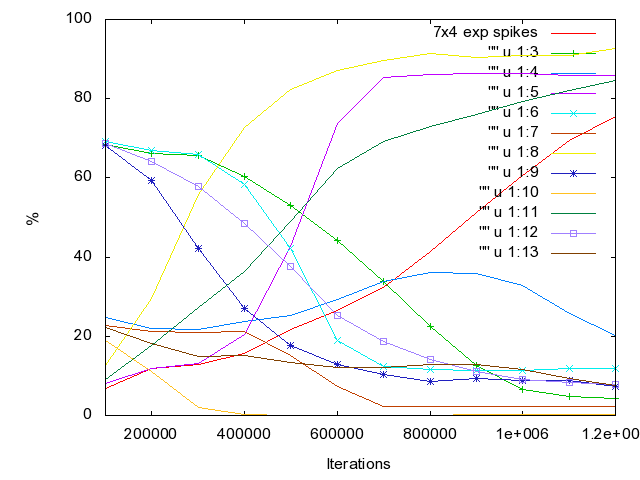
\includegraphics[width=0.4\textwidth]{7-4-exp-spikes}}\,
  \subfloat{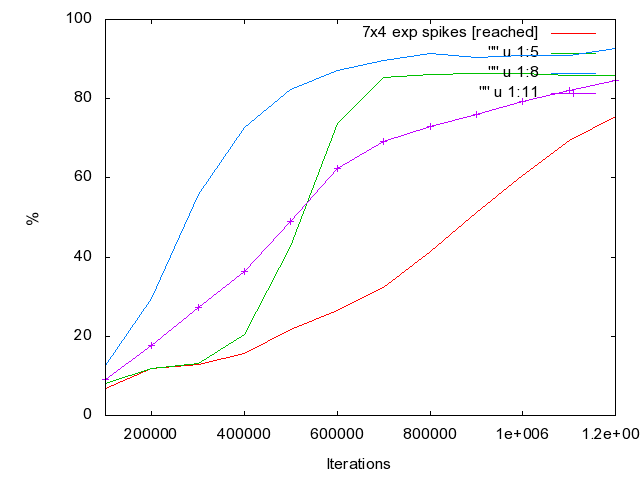
\includegraphics[width=0.4\textwidth]{7-4-exp-spikes_r}} \\
  \subfloat{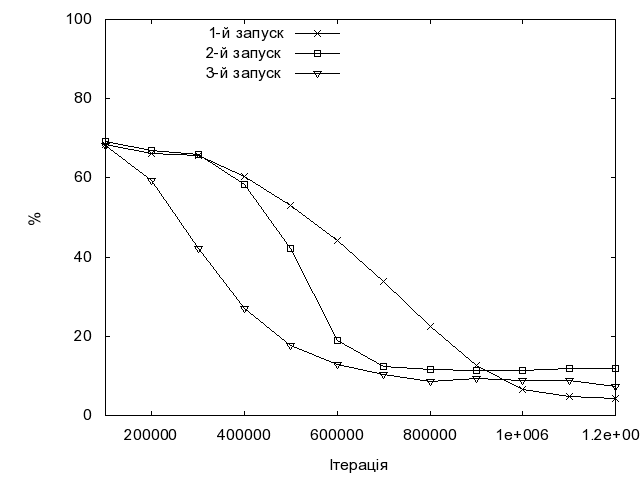
\includegraphics[width=0.4\textwidth]{7-4-exp-spikes_c}}\,
  \subfloat{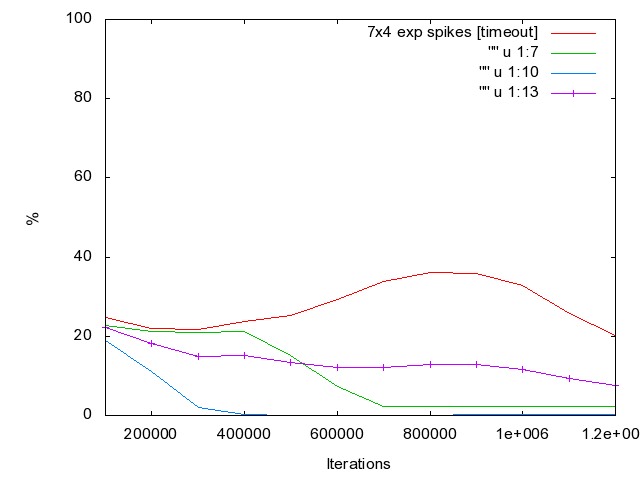
\includegraphics[width=0.4\textwidth]{7-4-exp-spikes_t}}
  \caption{7x4 exp spikes}
\end{figure}

\begin{figure}
  \centering
  \subfloat{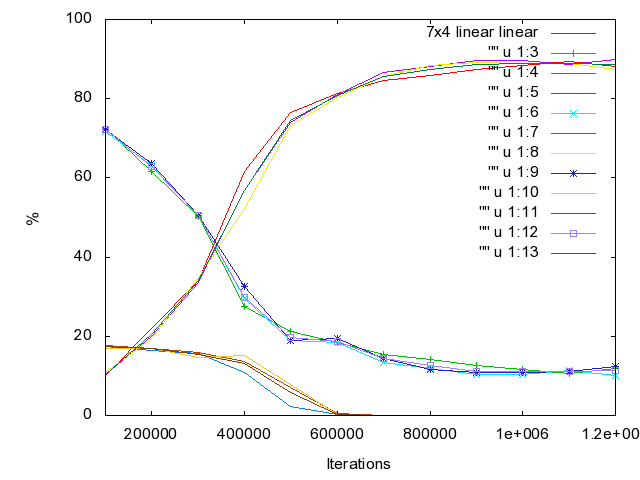
\includegraphics[width=0.4\textwidth]{7-4-linear-linear}}\,
  \subfloat{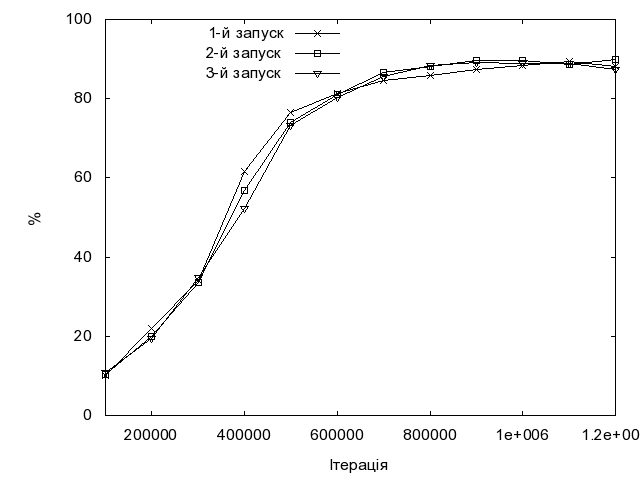
\includegraphics[width=0.4\textwidth]{7-4-linear-linear_r}} \\
  \subfloat{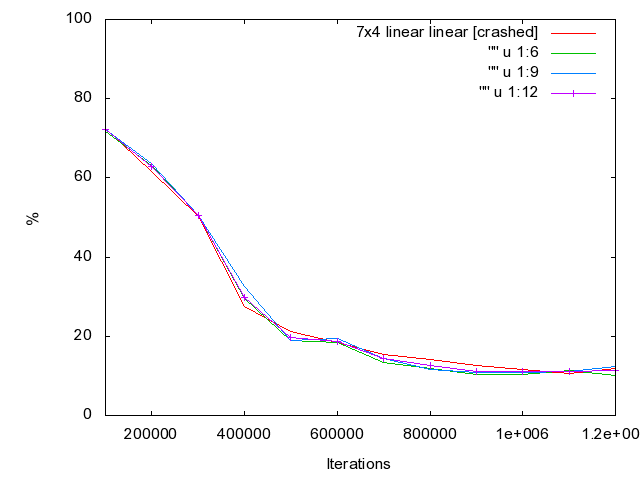
\includegraphics[width=0.4\textwidth]{7-4-linear-linear_c}}\,
  \subfloat{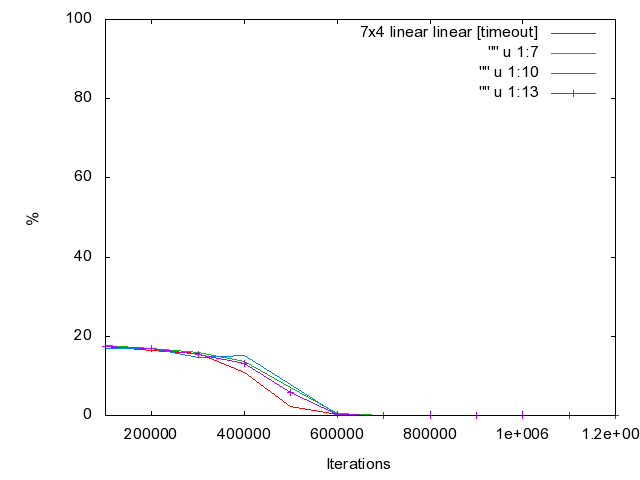
\includegraphics[width=0.4\textwidth]{7-4-linear-linear_t}}
  \caption{7x4 linear linear}
\end{figure}

\begin{figure}
  \centering
  \subfloat{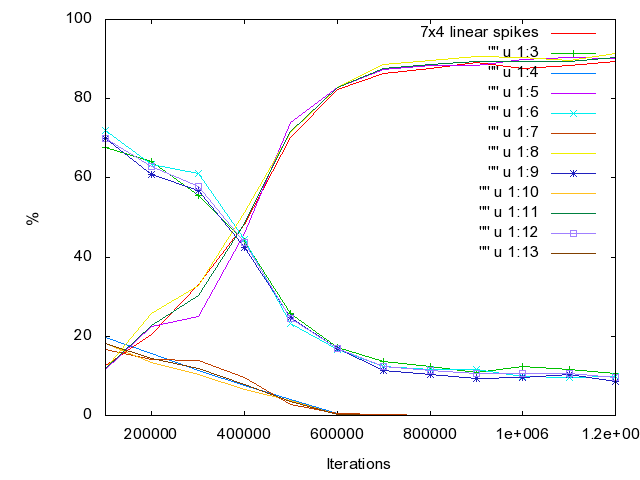
\includegraphics[width=0.4\textwidth]{7-4-linear-spikes}}\,
  \subfloat{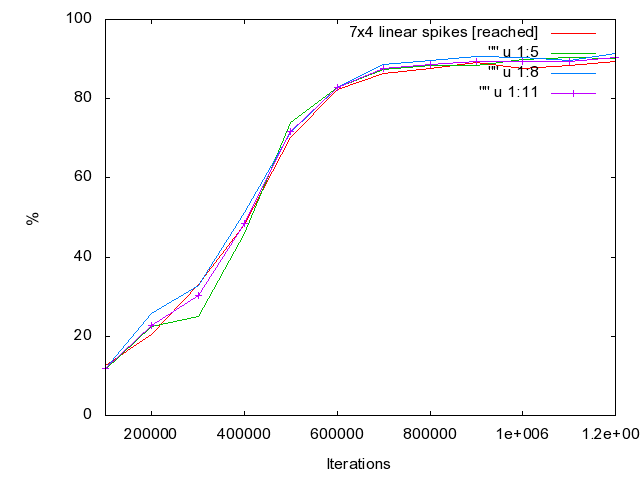
\includegraphics[width=0.4\textwidth]{7-4-linear-spikes_r}} \\
  \subfloat{\includegraphics[width=0.4\textwidth]{7-4-linear-spikes_c}}\,
  \subfloat{\includegraphics[width=0.4\textwidth]{7-4-linear-spikes_t}}
  \caption{7x4 linear spikes}
\end{figure}

\clearpage
\newpage

Цей тестовий набір включає нейромережі з архітектурами 3x2, 5x3 та 7x4 і покажує, що для успішного навчання достатньо найменшої з цих трьох нейромереж.
В усіх випадках використовувалися spikes-функції, як описані вище (погані).

\begin{figure}[h]
  \centering
  \subfloat{\includegraphics[width=0.4\textwidth]{3-2-s-s_s3}}\,
  \subfloat{\includegraphics[width=0.4\textwidth]{3-2-s-s_s3_r}} \\
  \subfloat{\includegraphics[width=0.4\textwidth]{3-2-s-s_s3_c}}\,
  \subfloat{\includegraphics[width=0.4\textwidth]{3-2-s-s_s3_t}}
  \caption{3x2 spikes spikes}
\end{figure}

\begin{figure}
  \centering
  \subfloat{\includegraphics[width=0.4\textwidth]{5-3-s-s_s3}}\,
  \subfloat{\includegraphics[width=0.4\textwidth]{5-3-s-s_s3_r}} \\
  \subfloat{\includegraphics[width=0.4\textwidth]{5-3-s-s_s3_c}}\,
  \subfloat{\includegraphics[width=0.4\textwidth]{5-3-s-s_s3_t}}
  \caption{5x3 spikes spikes}
\end{figure}

\begin{figure}
  \centering
  \subfloat{\includegraphics[width=0.4\textwidth]{7-4-s-s_s3}}\,
  \subfloat{\includegraphics[width=0.4\textwidth]{7-4-s-s_s3_r}} \\
  \subfloat{\includegraphics[width=0.4\textwidth]{7-4-s-s_s3_c}}\,
  \subfloat{\includegraphics[width=0.4\textwidth]{7-4-s-s_s3_t}}
  \caption{7x4 spikes spikes}
\end{figure}

\clearpage
\newpage

Тестові набори на виправлених функціях... повне розчарування :). Нейромережа --- 5x3.

$\varepsilon$-функція вибору випадкової дії: 
\begin{itemize}
\item \textbf{$\varepsilon$-spikes3} --- пилкоподібно-спадна з 3-ма зубцями спад від $0.3$ до $0.01$ за 600000 ітерацій;
\item \textbf{$\varepsilon$-spikes5} --- пилкоподібно-спадна з 5-ма зубцями спад від $0.4$ до $0.01$ за 1000000 ітерацій;
\end{itemize}

$\eta$-функція кроку навчання для нейромережі:
\begin{itemize}
\item \textbf{exp} ---    експоненційно-спадна від $0.5$ до $0.01$ за 1000000 ітерацій;
\item \textbf{spikes} --- пилкоподібно-спадна з 3-ма зубцями від $0.5$ до $0.01$ за 1000000 ітерацій;
\end{itemize}

\newpage
\begin{figure}
  \centering
  \subfloat{\includegraphics[width=0.4\textwidth]{suit-2009-12-26_5-3_test-case1}}\,
  \subfloat{\includegraphics[width=0.4\textwidth]{suit-2009-12-26_5-3_test-case1_r}} \\
  \subfloat{\includegraphics[width=0.4\textwidth]{suit-2009-12-26_5-3_test-case1_c}}\,
  \subfloat{\includegraphics[width=0.4\textwidth]{suit-2009-12-26_5-3_test-case1_t}}
  \caption{5x3 spikes $\varepsilon$-spikes3}
\end{figure}

\begin{figure}
  \centering
  \subfloat{\includegraphics[width=0.4\textwidth]{suit-2009-12-26_5-3_test-case2}}\,
  \subfloat{\includegraphics[width=0.4\textwidth]{suit-2009-12-26_5-3_test-case2_r}} \\
  \subfloat{\includegraphics[width=0.4\textwidth]{suit-2009-12-26_5-3_test-case2_c}}\,
  \subfloat{\includegraphics[width=0.4\textwidth]{suit-2009-12-26_5-3_test-case2_t}}
  \caption{5x3 spikes $\varepsilon$-spikes5}
\end{figure}

\begin{figure}
  \centering
  \subfloat{\includegraphics[width=0.4\textwidth]{suit-2009-12-26_5-3_test-case3}}\,
  \subfloat{\includegraphics[width=0.4\textwidth]{suit-2009-12-26_5-3_test-case3_r}} \\
  \subfloat{\includegraphics[width=0.4\textwidth]{suit-2009-12-26_5-3_test-case3_c}}\,
  \subfloat{\includegraphics[width=0.4\textwidth]{suit-2009-12-26_5-3_test-case3_t}}
  \caption{5x3 exp $\varepsilon$-spikes3}
\end{figure}

\begin{figure}
  \centering
  \subfloat{\includegraphics[width=0.4\textwidth]{suit-2009-12-26_5-3_test-case4}}\,
  \subfloat{\includegraphics[width=0.4\textwidth]{suit-2009-12-26_5-3_test-case4_r}} \\
  \subfloat{\includegraphics[width=0.4\textwidth]{suit-2009-12-26_5-3_test-case4_c}}\,
  \subfloat{\includegraphics[width=0.4\textwidth]{suit-2009-12-26_5-3_test-case4_t}}
  \caption{5x3 exp $\varepsilon$-spikes5}
\end{figure}

\clearpage
\newpage

Параметри ближчі до першого випадку, тільки нейромережа --- 5x3, а функції виправлені на правильні.

$\varepsilon$-функція вибору випадкової дії: 
\begin{itemize}
\item \textbf{$\varepsilon$-spikes3} --- пилкоподібно-спадна з 3-ма зубцями спад від $0.3$ до $0.01$ за 600000 ітерацій;
\item \textbf{$\varepsilon$-spikes5} --- пилкоподібно-спадна з 5-ма зубцями спад від $0.4$ до $0.01$ за 1000000 ітерацій;
\end{itemize}

$\eta$-функція кроку навчання для нейромережі:
\begin{itemize}
\item \textbf{exp} ---    експоненційно-спадна від $0.4$ до $0.01$ за 600000 ітерацій;
\item \textbf{spikes} --- пилкоподібно-спадна з 3-ма зубцями від $0.4$ до $0.01$ за 600000 ітерацій;
\end{itemize}

\newpage

\begin{figure}
  \centering
  \subfloat{\includegraphics[width=0.4\textwidth]{suit-2009-12-26_5-3-conservative_test-case1}}\,
  \subfloat{\includegraphics[width=0.4\textwidth]{suit-2009-12-26_5-3-conservative_test-case1_r}} \\
  \subfloat{\includegraphics[width=0.4\textwidth]{suit-2009-12-26_5-3-conservative_test-case1_c}}\,
  \subfloat{\includegraphics[width=0.4\textwidth]{suit-2009-12-26_5-3-conservative_test-case1_t}}
  \caption{5x3 spikes $\varepsilon$-spikes5}
\end{figure}

\begin{figure}
  \centering
  \subfloat{\includegraphics[width=0.4\textwidth]{suit-2009-12-26_5-3-conservative_test-case2}}\,
  \subfloat{\includegraphics[width=0.4\textwidth]{suit-2009-12-26_5-3-conservative_test-case2_r}} \\
  \subfloat{\includegraphics[width=0.4\textwidth]{suit-2009-12-26_5-3-conservative_test-case2_c}}\,
  \subfloat{\includegraphics[width=0.4\textwidth]{suit-2009-12-26_5-3-conservative_test-case2_t}}
  \caption{5x3 spikes $\varepsilon$-spikes3}
\end{figure}

\begin{figure}
  \centering
  \subfloat{\includegraphics[width=0.4\textwidth]{suit-2009-12-26_5-3-conservative_test-case3}}\,
  \subfloat{\includegraphics[width=0.4\textwidth]{suit-2009-12-26_5-3-conservative_test-case3_r}} \\
  \subfloat{\includegraphics[width=0.4\textwidth]{suit-2009-12-26_5-3-conservative_test-case3_c}}\,
  \subfloat{\includegraphics[width=0.4\textwidth]{suit-2009-12-26_5-3-conservative_test-case3_t}}
  \caption{5x3 exp $\varepsilon$-spikes5}
\end{figure}

\begin{figure}
  \centering
  \subfloat{\includegraphics[width=0.4\textwidth]{suit-2009-12-26_5-3-conservative_test-case4}}\,
  \subfloat{\includegraphics[width=0.4\textwidth]{suit-2009-12-26_5-3-conservative_test-case4_r}} \\
  \subfloat{\includegraphics[width=0.4\textwidth]{suit-2009-12-26_5-3-conservative_test-case4_c}}\,
  \subfloat{\includegraphics[width=0.4\textwidth]{suit-2009-12-26_5-3-conservative_test-case4_t}}
  \caption{5x3 exp $\varepsilon$-spikes4}
\end{figure}

\end{document}
